\section{Theory}
\subsection{Theoretical Exercises}
\subsubsection[Origin of the 21 cm HI-Line]{Origin of the \SI{21}{cm} \ce{H_I}-Line}
The \SI{21}{cm} \ce{H_I}-Line refers to electromagnetic radiation emitted from atomic hydrogen. It has a wavelength of \SI{21.11}{cm} (that is \SI{1420.03}{\mega\hertz}) \cite[Ch 3.1]{srt}.

This emission is caused by a transition from the $\ce{S_{\frac{1}{2}}(F=1)}$ to the $\ce{S_{\frac{1}{2}}(F=0)}$ state, meaning that the nuclear spin and electron spin transition from parallel to antiparallel.
The $\ce{S_{\frac{1}{2}}(F=1)}$ state has a half-life of about 8 million years, but the line is observable due to the large column density of atomic hydrogen in the interstellar medium. \cite[Ch. 13.1]{wilson_tools_2009}

The main reason for interest in specifically this frequency is the aforementioned atomic hydrogen, but there are other sources that can emit at this wavelength, some of them are: \cite[11.1-11.4]{wilson_tools_2009}
\begin{itemize}
    \item The sun
    \item Thermal radiation from molecular hydrogen
    \item Ionized stellar winds
    \item Supernovae
\end{itemize}
\subsubsection{Angular resolution of the SRT}\label{sec:ang_res}
Using the equation relating the effective area $A_e$ and the wavelength $\lambda$ \cite[p. 149]{wilson_tools_2009}
\begin{equation}
    A_e \Omega_A = \lambda^2
\end{equation}
and the definitions of the effective area and the geometric area \cite[p. 148]{wilson_tools_2009}
\begin{equation}
    A_e = \eta A_g \qquad A_g = \pi \left( \frac{d}{2} \right)^2 \label{eq:A_e}
\end{equation}
we can then solve for the antenna beam solid angle.
\begin{equation}
    \Omega_A = \frac{\lambda^2}{A_g \eta} \label{eq:Omega_A}
\end{equation}


To compute an approximation of the full width at half maximum $\theta$ (FWHM) we can approximate the aperture as gaussian \cite[p. 2]{srt} and note the following properties.
\begin{equation}
    \Omega_A \approx \int_{4\pi } d\Omega\, \exp{\left( -\frac{\vartheta^2}{2\sigma^2} \right)} \approx 2\pi \int_0^{\infty} d\vartheta \, \vartheta \exp{\left( -\frac{\vartheta^2}{2\sigma^2} \right)} = 2\pi \sigma^2
    \label{eq:gauss_integral}
\end{equation}
\begin{equation}
    \exp{\left( -\frac{(\theta/2)^2}{2\sigma^2}\right)} = \frac{1}{2} \quad \implies \quad \theta = 2 \sqrt{2\ln{2}} \sigma \label{eq:fwhm_sigma}
\end{equation}
using Eq. \eqref{eq:gauss_integral} and Eq. \eqref{eq:fwhm_sigma} we can solve for $\Omega_A$ in terms of $\theta$
\begin{equation}
    \Omega_A = \frac{\pi}{4\ln{2}} \theta^2 \approx 1.133 \, \theta^2 \label{eq:Omega_A_fwhhm}
\end{equation}
Notice that this is consistent with \cite[Eq. (8.13)]{wilson_tools_2009}

Equating Eq. \eqref{eq:Omega_A} and Eq. \eqref{eq:Omega_A_fwhhm} and then solving for $\theta$ we get an expression for the expected FWHM.
\begin{equation}
    \theta = \frac{4}{\pi} \sqrt{\frac{\ln{2}}{\eta}}\frac{\lambda}{d} \label{eq:fwhm}
\end{equation}

To compute the FWHM we need the diameter of the SRT which is $d = \SI{4}{m}$ \cite[p. 4]{srt}, and the antenna efficiency which is $\eta = 0.5$ \cite[p. 2]{srt}.
Unfortunately we cannot reasonably estimate an error for the antenna efficiency $\eta$, we suspect however that the error of the antenna efficiency dominates here.
Therefore we will waive a proper error discussion at this point, and work with exact values.

We can then obtain the values shown in Table \ref{tab:ang_res}.
\begin{table}[H]
    \centering
    \begin{tabular}{rrrr}
        \toprule
        FWHM $\theta$ [\si{\degree}] & Wavelength $\lambda$ [\si{cm}] & Frequency [\si{\giga \hertz}]\\
        \midrule
        \num{4.533} & \num{21.11} & \num{1.420}\\
        \num{0.688} & \num{0.30} & \num{10.000}\\
        \bottomrule
    \end{tabular}
    \caption{Angular resolution of the SRT at different frequencies}
    \label{tab:ang_res}
\end{table}
\subsubsection{Antenna, brightness and noise temperature}

The spectral radiance of a black body can be described by the Rayleigh-Jeans law for low frequencies ($\nu \ll T$) \cite[Eq. (3)]{srt}
\begin{equation}
    I_\nu = \frac{2\nu^2}{c^2}k_{B}T \label{eq:rayleigh_jeans}
\end{equation}
Using Eq.~\eqref{eq:rayleigh_jeans}, the brightness temperature $T_B$ can be defined as the temperature that produces the observed spectral radiance at a given frequency:
\begin{equation}
    T_B = \frac{c^2}{2\nu^2k_{B}} I_\nu
\end{equation}

An antenna measures power rather than intensity. The received spectral power is given by
\begin{equation}
    P_\nu = A_e I_\nu,
\end{equation}
where $A_e$ is the effective area of the antenna. Substituting $I_\nu$ from Eq.~\eqref{eq:rayleigh_jeans} yields
\begin{equation}
    P_\nu = A_e \frac{2\nu^2 k_B}{c^2} T_B.
\end{equation}

The antenna response is not uniform over the sky but described by the normalized antenna pattern $P_n(\theta, \phi)$,
\begin{equation}
    \int_{4\pi} P_n(\theta, \phi) \, d\Omega = 1.
\end{equation}
The antenna temperature $T_A$ is defined as the equivalent brightness temperature that would produce the same received power as the actual sky brightness distribution $T_B(\theta, \phi)$:
\begin{equation}
    T_A = \int_{4\pi} P_n(\theta, \phi) \, T_B(\theta, \phi) \, d\Omega.
\end{equation}
It represents the sky-averaged brightness temperature weighted by the antenna beam pattern.

In addition to the sky signal, the receiver introduces intrinsic noise, characterized by the noise temperature $T_N$. The total system noise, expressed as the system temperature, is then
\begin{equation}
    T_\text{sys} = T_A + T_N.
\end{equation}

\subsubsection{Temperature conversion}\label{sec:antenna_temp}
The goal is to find a way to compute the antenna temperature from the voltage output of the spectrometer.
It is important to note that this voltage is proportional to power received by the antenna and thus proportional to the antenna temperature.
Because of this linear relationship it is possible to relate the gain $G$, voltage output $U$, noise temperature $T_N$ and antenna temperature $T_A$. \cite[Eq. (5)]{srt}
\begin{equation}
    U(T_A) = G(T_A + T_N) \label{eq:U_from_T}
\end{equation}
What is now left is to find a procedure to determine $G$ and $T_N$. This is done by observing two different radiation sources which will result in known antenna temperatures. Let's call these temperatures $T_\text{hot}$ and $T_\text{cold}$ and their resulting voltages $U_\text{hot}$ and $T_\text{cold}$ respectively.
With these measurements it is now easy to find the relevant expressions for $G$ and $T_N$.
We can then use Eq. \eqref{eq:U_from_T} to build a linear system of equations with the measured values.
\begin{equation} \label{eq:P_to_Ta_sys}
	\begin{split}
		U_\text{cold} &= G \cdot (T_\text{cold} + T_N) \\
		U_\text{hot} &= G \cdot (T_\text{hot} + T_N)
	\end{split}
\end{equation}
The only unknown quantities are then the noise temperature $T_N$ with units [K] and the gain of the instrument $G$ with units [V/K].
These can be solved for.
\begin{align}
	G &= \frac{U_h-U_c}{T_h-T_c}\label{eq:G}\\
	T_N &= \frac{T_h U_c-T_c U_h}{U_h-U_c}\label{eq:TN}
\end{align}
Because the parameters $G$ and $T_N$ can change over time it is important to frequently calibrate the antenna. The procedure can also fail if the sources of the known temperatures are not reliable, or if the assumption that the relationship between the output voltage and the antenna temperature is linear does not hold.

\subsubsection{Expected temperature of the sun}\label{sec:sun_temp}
We might naively expect the brightness temperature of the sun to be equal to its surface temperature $T_{\odot} = \SI{5778}{\kelvin}$ \cite[p. 211]{durandi_formeln_2011}. But this is wrong, because the sun doesn't behave itself like a black body at these frequencies.
In Figure \ref{fig:sun_temp_theory} we can see, that the sun has a brightness temperature of 100'000 \si{\kelvin} up to 10 million \si{\kelvin}.
\begin{figure}[H]
    \centering
    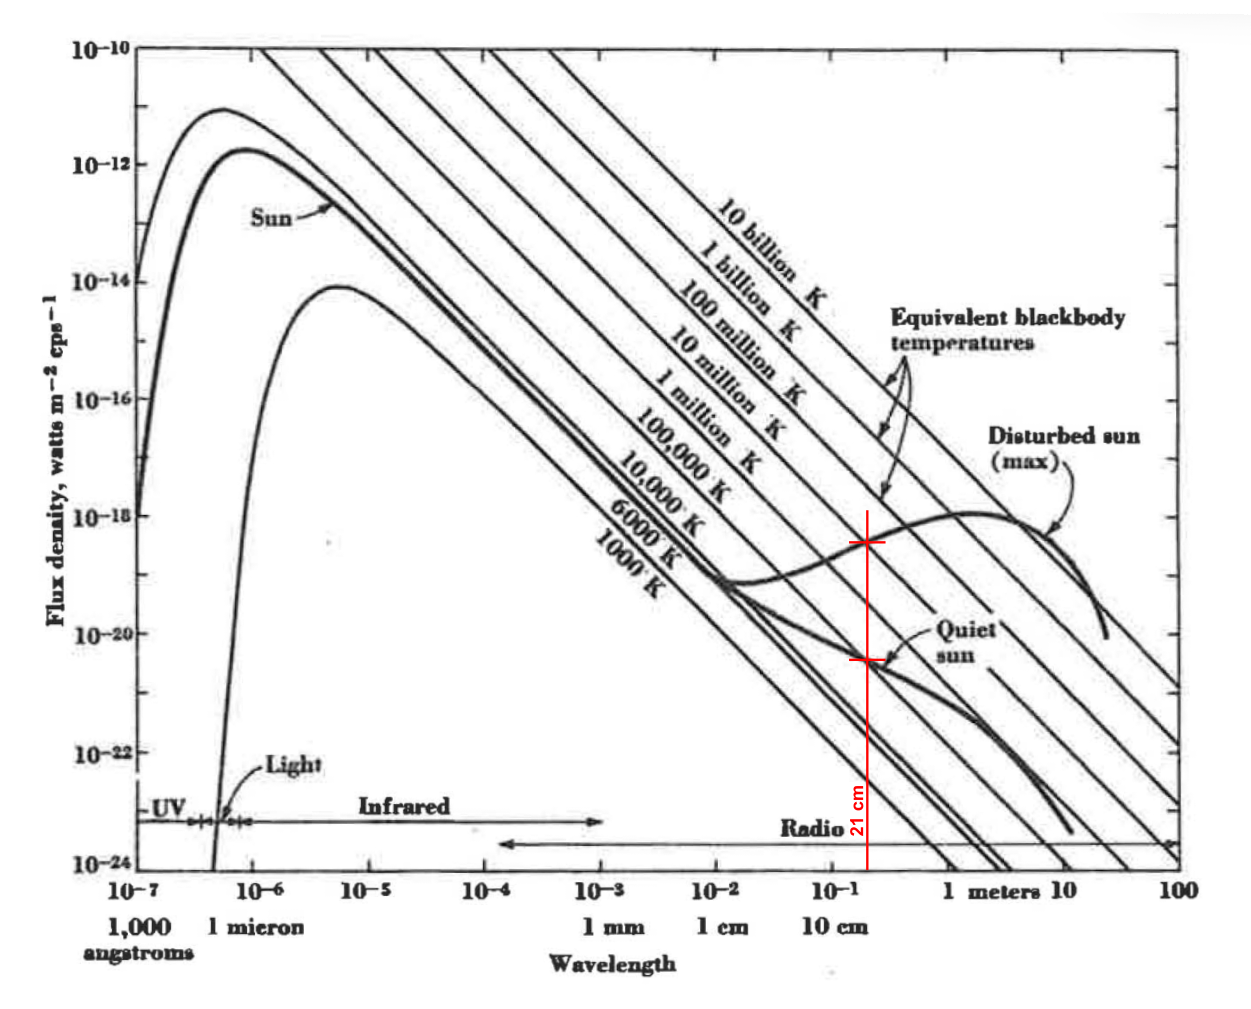
\includegraphics[width=0.6\textwidth]{assets/SunBrightnessTheory.png}
    \caption{Wavelength dependence of the Brightness temperature of the sun \cite[p.8-45 Fig. 8-34]{kraus_radio_1986}}
    \label{fig:sun_temp_theory}
\end{figure}

\subsubsection{Influence of elevation angle}
At a frequency of \SI{1.42}{\giga\hertz} we don't expect a significant influence of the elevation angle on the measured brightness temperature, since the atmosphere is transparent at this wavelength.
The frequency of \SI{22}{\giga\hertz} is however very close to an absorption band caused by water vapor \ce{H_2O} at \SI{22.2}{\giga\hertz}.
We can make a reasonable but naive model of the attenuation at this frequency by considering that the attenuation is exponential in the distance traveled through the atmosphere.
Ignoring the curvature of the earth, the distance traveled through the atmosphere can be computed trigonometrically. We can then model the transmission coefficient $\tau$ with Eq.\eqref{eq:attenuation}.
\begin{equation}
    \tau = C_1 \exp{\left( - C_2 \frac{1}{\abs{\cos{\theta}}} \right)} \label{eq:attenuation}
\end{equation}
Where $C_1$ and $C_2$ depend on the absorption coefficient of \ce{H_2O} at \SI{22.2}{\giga\hertz} and the thickness of the atmosphere.



\subsubsection{Doppler shift}

\subsection{Rotation of the Milky Way}
